\chapter{Introduction}

In the most general sense, this research strives to create
autonomous computational methods to 
\begin{itemize}
\item {\bf See} axial cross-sections of CT/MR scans (computer vision), 
\item {\bf Classify} what is seen into basic human anatomy categories (recognition, deep learning), and
\item {\bf Build} geometric representations of these anatomies into domains (e.g., 
voxels, meshes, analytical geometry) suitable for computational analysis (e.g., 
finite element analysis, finite volume analysis).
\end{itemize}
In a sense, we wish to combine the skills of a radiologist and an engineer
into an automated workflow that can be performed by a computer.  

The overarching goal of this effort is to push toward highly personalized
medicine, wherein the individual's anatomical geometry, derived from an imaging
series, is reconstructed into a high-fidelity, three dimensional (3D) 
geometric model suitable not only for visualization but also for 
analysis of a personal response to a mechanically deleterious environment, 
such as blast, blunt, or ballistic exposure.  Common examples of these 
environments include slip-and-fall accidents and automobile collisions.  
Less frequent, but particularly relevant to the U.S.~warfighter, is exposure
to blast overpressure from improvised explosive devices (IEDs) and 
fragmentation.  

In the subsequent sections, we present an overview of the topics covered
in this manuscript, followed by details of each.

\section{Overview}
To come.

\section{Motivation by Analogy}

The concept of converting pixels to a geometric representation, hereinafter
referred to as PTG (Pixel To Geometry), can be introduced 
by consideration of two similar processes, optical character recognition (OCR) 
and analytic geometry.

OCR is the process of converting pixel values scanned from a piece of paper with
printed or handwritten text into a digital encoding of letters and
number, e.g., 
\begin{equation*}
\mbox{\tt A a B b C c } \ldots\; \mbox{\tt Z z 0 1 2 3 4 5 6 7 8 9},
\end{equation*}
where a collection of pixels is composed to map to letters and numbers.

Figure~\ref{fig:geometry_pixels} illustrates the difference between vector
graphics and rasterized graphics. 
The word ``geometry'' appearing with font 
size 48~point (72 points = 1 inch) composed of 
vector graphics, and the ``e'' in yellow, with font size 72~point, 
appearing from left-to-right 
at half-inch intervals in rasterized 
graphics at 10 pixels per inch (ppi), 20 ppi, 40 ppi, and 80 ppi.  The 
image was saved in vectorized format at 600 ppi.
\\ \\ % not sure why we need to extra bump space to move the figure down?
\begin{figure}[htb]
  \begin{center}
    % 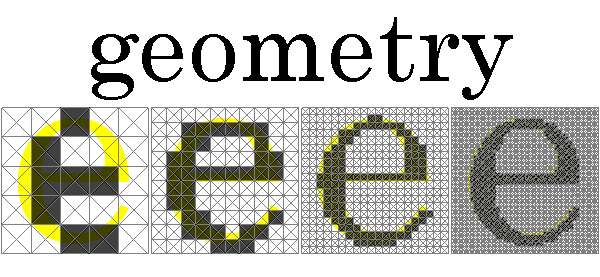
\includegraphics[width=\textwidth]{fig/geometry.pdf}
    % \begin{overpic}[width=0.62\textwidth, abs, grid, unit=0.5in, tics=1]{fig/geometry.pdf}
    % \begin{overpic}[width=0.62\textwidth, abs, unit=0.5in, tics=1]{fig/geometry.pdf}
    % \begin{overpic}[width=0.8\textwidth, abs, grid, unit=0.5in, tics=1]{fig/geometry.pdf}
    \begin{overpic}[width=0.8\textwidth, abs, unit=0.5in, tics=1]{fig/geometry.pdf}
      \put(1.15, 0){10 ppi}
      \put(3.65, 0){20 ppi}
      \put(6.15, 0){40 ppi}
      \put(8.65, 0){80 ppi}
    \end{overpic}
  \end{center}
    \caption{Illustration of vector graphics versus rasterized graphics, and the
    concept of pixel resolution.
    Reference: fig/geometry.pdf}
  \label{fig:geometry_pixels} % label must come after caption 
\end{figure}

